\documentclass{beamer}

%%% Imports
\usetheme{CambridgeUS}
\usepackage{graphicx}
\usepackage[normalem]{ulem}

%%% Headline template
\setbeamertemplate{headline}
{
  \leavevmode%
  \hbox{%
  \begin{beamercolorbox}[wd=.55\paperwidth,ht=4ex,dp=1.5ex,center]{section in head/foot}%
    \usebeamerfont{section in head/foot} A difficulty in the concept of social welfare
  \end{beamercolorbox}%
  
  \begin{beamercolorbox}[wd=.45\paperwidth,ht=4ex,dp=1.5ex,center]{subsection in head/foot}%
    \usebeamerfont{subsection in head/foot} \insertsubsectionhead
  \end{beamercolorbox}}%
  \vskip0pt%
}

%%% Footline template
\setbeamertemplate{footline}
{
  \leavevmode%
  \hbox{%
  \begin{beamercolorbox}[wd=.333333\paperwidth,ht=2.25ex,dp=1ex,center]{author in head/foot}%
    \usebeamerfont{author in head/foot}\insertshortauthor
  \end{beamercolorbox}%
  
  \begin{beamercolorbox}[wd=.333333\paperwidth,ht=2.25ex,dp=1ex,center]{title in head/foot}%
    \usebeamerfont{title in head/foot}\insertshortinstitute
  \end{beamercolorbox}%
  
  \begin{beamercolorbox}[wd=.333333\paperwidth,ht=2.25ex,dp=1ex,right]{date in head/foot}%
    \usebeamerfont{date in head/foot}\insertshortdate{}\hspace*{2em}
    \insertframenumber{} / \inserttotalframenumber\hspace*{2ex} 
  \end{beamercolorbox}}%
  \vskip0pt%
}

%%% Definitions
\title[A difficulty in the concept of social welfare]{A difficulty in the concept of social welfare}
\author[Mario Sguario]{Kenneth J. Arrow}
\institute[University of Trento]{Stanford University}
\date[Jun 3, 2026]{Aug, 1950}
\logo{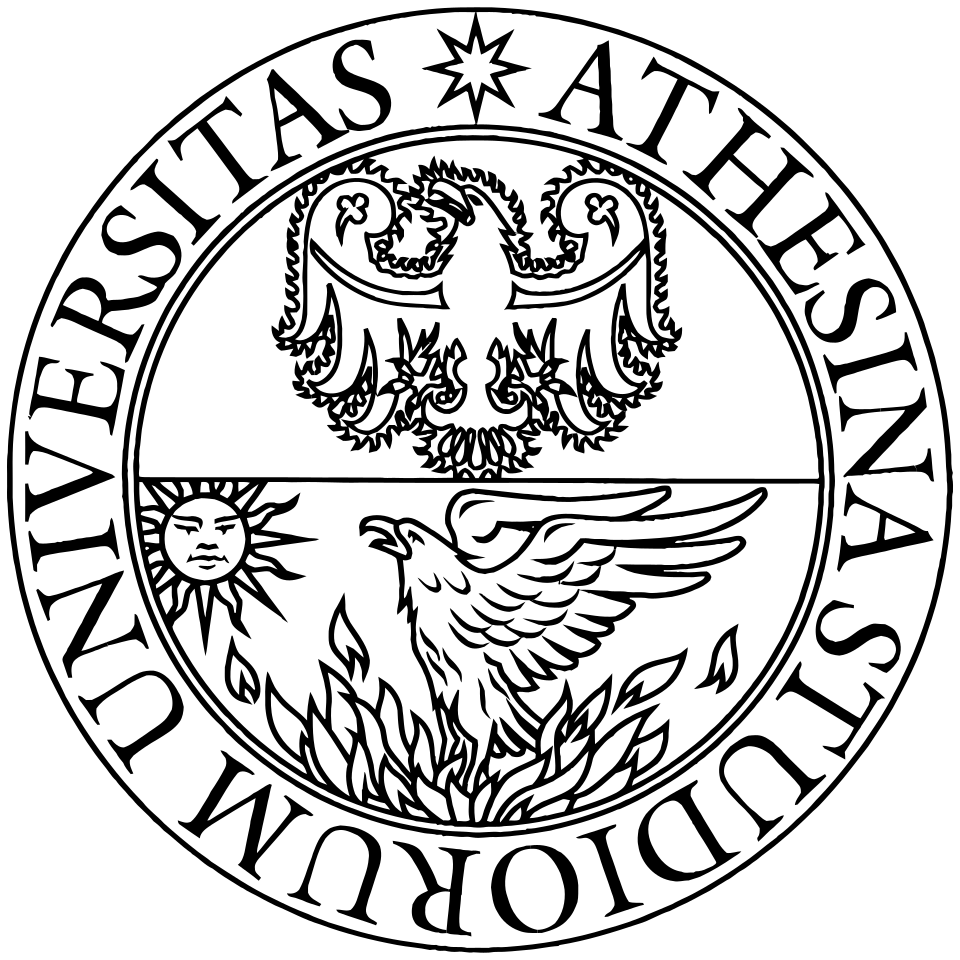
\includegraphics[height=0.5cm]{uni.png}}

%%% Slideshow
\begin{document}

\begin{frame}
    \titlepage
\end{frame}

%%%%-------------------------------------------------------------------------
\subsection{Introduction}
\begin{frame}{Introduction}
 Arrow defines two ways to make social choices in a capitalist democracy:
    \begin{itemize}    
    \item \textbf{Voting} (for political decisions)
    \item \textbf{The Market Mechanism} (for economic decisions)
    \end{itemize}
\end{frame}

\begin{frame}{Introduction}
 It also defines two ways to make choices based on a single entity, ideally respecting a single common will:
    \begin{itemize}
        \item \textbf{Dictatorship:} The social preference is determined entirely by the preferences of a single individual.
        \item \textbf{Convention:} Collective choices are dictated by a divine or commonly shared will.
    \end{itemize}
    \vspace{0.5cm}
     In these societies, \textbf{there are no conflicting choices}: \\
     \vspace{0.25cm}
     \begin{itemize}
        \item[$\Rightarrow$] \underline{Any single entity can be rational in his choice.}
    \end{itemize}
\end{frame}

\begin{frame}{The Core Problem}
    \begin{itemize}
        \item \textbf{How can we aggregate individual preferences into a collective, \uline{rational} social choice?}
        \begin{itemize}
            \item[$\Rightarrow$] We need to define a \textbf{social welfare function}
        \end{itemize}
        \vspace{0.25cm}
        \item Traditional democratic methods, often fail..
        \begin{itemize}
            \item Majority Decision
            \item Pareto optimum
            \item Compensation Principle
        \end{itemize}
    \end{itemize}
\end{frame}

\begin{frame}{Majority decision}
    \textbf{The Paradox of Voting:}\\
      It shows that even if every individual has rational, consistent preferences, the \textit{collective} social preference can be irrational.
    \vspace{0.5cm}
    \begin{itemize}
        \item Three voters (1, 2, 3) ranking three options (A, B, C):
        \begin{enumerate}
            \item $A > B > C$
            \item $B > C > A$
            \item $C > A > B$
        \end{enumerate}
        \item \textbf{The Majority Result:} 
        \begin{itemize}
            \item A is preferred over B
            \item B is preferred over C
        \end{itemize}
        \item[$\Rightarrow$] Logically, A should be preferred over C; however:
        \begin{itemize}
            \item C is preferred over A $\rightarrow$ \textbf{Paradox}
        \end{itemize}
    \end{itemize}
\end{frame}

\begin{frame}{Welfare economics}
    {\setlength{\leftskip}{0.9cm}}
    If we view rationality as a maximization process, the challenge of achieving a \textit{social maximum} coincides with the central problem of welfare economics.
    \vspace{0.25cm}
    \begin{itemize}
        \item \textbf{Goal:} Maximize social utility
        \vspace{0.25cm}
        \item \textbf{Weaker goal:} Pareto optimum
        \vspace{0.25cm}
        \begin{itemize}
            \item This solution still has problems:
            \begin{enumerate}
                \item Redistribution problem
                \item Preservation of Status Quo
                \item No social indifference map $\rightarrow$ No prescription for actions
            \end{enumerate}
        \end{itemize}
    \end{itemize}
\end{frame}


\begin{frame}{Compensation principle}
    When choosing between 2 economic states \textit{x} and \textit{y}, \textit{x} should be preferred over \textit{y} if there is a method of paying compensations under \textit{x} so that everybody is made better off than they are in state \textit{y}.
    \vspace{0.25cm}
    \begin{itemize}
        \item \textbf{Paradox:} It is possible that \textit{x} is preferred over \textit{y} and vice versa.
        \item Even without the paradox occurring \uline{it fails to produce a linear ordering of social choices.}
    \end{itemize}
\end{frame}

\begin{frame}{A general problem}
        The aim of the paper is to show that the difficulties seen in voting and economics are general:
        \begin{itemize}
            \item For any methods of deriving social choices by aggregating individual preference patterns $\rightarrow$ it is possible to find individual preference patterns that create a social choice which does not have a linear ordering.
            \item It is assumed that each individual behaves rationally $\rightarrow$ his behavior can be described by an indifference map.
        \end{itemize}
\end{frame}

%%%%-------------------------------------------------------------------------
\subsection{Definitions and Notation}
\begin{frame}{Basic definitions}
    \begin{itemize}
        \item We define a set of mutually exclusive alternatives denoted by small letters, \textit{x, y, z...}
        \item A \textit{subset S} over the \textit{Set} contains the voting alternatives.
        \item User can only express a preference on a single pair of alternatives.
        \item Given a pair \textit{x, y} the chooser can express 3 possible choices:
        \begin{enumerate}
            \item Prefers \textit{x} over \textit{y}
            \item Neither \textit{x} or \textit{y} is preferred over the other 
            \item Prefers \textit{y} over \textit{x}
        \end{enumerate}
        \vspace{0.25cm}
        \item To simplify relations between alternatives a single relation is defined:
        \textit{xRy} $\rightarrow$ x is preferred or indifferent to y
        
    \end{itemize}
\end{frame}

\begin{frame}{The decision Protocol}
    \begin{itemize}
        \item The chooser evaluates all possible pairs of alternatives to establish a global preference scale, without yet knowing the opportunity set \textit{S}.
        \item Once the subset \textit{S} is revealed, the chooser picks the alternative that ranks highest according to their prior ordering.
        \vspace{0.25cm}
        \item \underline{Decisions are assumed to be consistent with one another.}
        \begin{itemize}
            \item If x preferred over y and y over z then x must be preferred over z.
            \item If x indifferent to y and y to over z then x must be indifferent to z.
        \end{itemize}
    \end{itemize}
\end{frame}

\begin{frame}{Axiom I, II}

    \begin{itemize}
        \item \textbf{Axiom I:} For all \textit{x} and \textit{y}, either \textit{xRy} or \textit{yRx}.
        \begin{itemize}
            \item Note that: both \textit{xRy} and \textit{yRx} can hold at the same time $\rightarrow$ \textit{x} is indifferent to \textit{y}.
            \item It holds even if \textit{(x = y)} implying \textit{xRx}.
        \end{itemize}
        \vspace{0.5cm}
        \item \textbf{Axiom II:} For all \textit{x}, \textit{y}, and \textit{z}, \textit{xRy} and \textit{yRz} imply \textit{xRz}.
        \begin{itemize}
            \item Guarantees transitivity, hence consistency.
            \item Alongside with Axiom I guarantees weak ordering.
        \end{itemize}
    \end{itemize}
\end{frame}

\begin{frame}{Definition I, II}
    \begin{itemize}
        \item \textbf{Definition I:} The notation \textit{xPy} is defined to mean not \textit{yRx}. 
        \begin{itemize}
            \item It is read as "\textit{x} is preferred to \textit{y}".
        \end{itemize}
        \vspace{0.5cm}
        \item \textbf{Definition II:} The notation \textit{xIy} it means \textit{xRy} and \textit{yRx} 
        \begin{itemize}
            \item It is read as "\textit{x} is indifferent to \textit{y}"
        \end{itemize}
        \vspace{0.5cm}
         \item We can now define 6 very intuitive \textbf{Lemmas:}
            \begin{itemize}
                \item \textbf{a:} For all \textit{x}, \textit{xRx}.
                \item \textbf{b:} If \textit{xPy}, then \textit{xRy}.
                \item \textbf{c:} If \textit{xPy} and \textit{yPz}, then \textit{xPz}.
                \item \textbf{d:} If \textit{xIy} and \textit{yIz}, then \textit{xIz}.
                \item \textbf{e:} For all \textit{x} and \textit{y}, either \textit{xRy} or \textit{yPx}.
                \item \textbf{f:} If \textit{xPy} and \textit{yRz}, then \textit{xPz}.
            \end{itemize}
            
        \end{itemize}
\end{frame}

\begin{frame}{The Mechanics of Rational Choice}
    \begin{itemize}
        \item \textbf{Clear Terminology:} To avoid mathematical ambiguity:
        \begin{itemize}
            \item \textit{R} is defined strictly as a \textbf{"weak ordering"}.
            \item \textit{P} is defined strictly as a \textbf{"preference relation"}.
        \end{itemize}
        \vspace{0.5cm}
        \item \textbf{Reduction to Pairs:} A rational individual's choice from \textit{any} collection of alternatives can be entirely determined just by knowing their choices between simple pairs.
    \end{itemize}
\end{frame}

\begin{frame}{The Ordering of social states}
    The objects of  collective choice are \underline{Social States.}
    \begin{itemize}
        \vspace{0.5cm}
        \item A \textbf{social state} is a complete description that includes: 
        \begin{enumerate}
            \item The amount of commodities in the hands of each individual
            \item The labor applied by each individual
            \item The amount of resources invested in each activity
            \item Each diplomatic and collective activity
        \end{enumerate}
        \begin{itemize}
            \item[$\Rightarrow$] Basically a snapshot of the whole society.
        \end{itemize}
        \item Each citizen has a definite ordering of all conceivable social states which they can order by whatever standards they deem relevant.
    \end{itemize}
\end{frame}

\begin{frame}{Tastes vs Values}
    Arrow overcomes pure individualism by distinguishing between \textbf{Tastes} and \textbf{Values} of each individual.
    \vspace{0.5cm}
    \begin{itemize}
        \item The Market takes into account only the ordering according to tastes, which cannot result in a true social maximum.
        \item Each preference of an individual should be considered, even the ones that do not directly relate to him.
        \begin{itemize}
            \item[$\Rightarrow$] Deciding whether a specific preference is relevant to society or simply "none of one's business" is, in itself, a value judgment. Thus, society must consider the entire system of values.
        \end{itemize}
    \end{itemize}
\end{frame}

\begin{frame}{Notation for social states}
    \begin{itemize}
        \item We define the ordering relation of social states of an individual \textit{i} with $R_i$, from which $P_i$ (strict preference) and $I_i$ (indifference) are derived.
        \vspace{0.5cm}
        \item Similarly, we define the whole society global social ordering relation with $R$, from which social preference $P$ and indifference $I$ are derived.
        \vspace{0.5cm}
        \item \textbf{The Aim of the Theorem} is to construct an $R$ that also reflects rational choice-making $\rightarrow$ $R$ satisfies Axioms I and II.
    \end{itemize}
\end{frame}

%%%%-------------------------------------------------------------------------
\subsection{The social welfare function}
\begin{frame}{Social welfare function}
    \framesubtitle{Bergson's Formulation}
    \begin{itemize}
        \item[$\Rightarrow$] Bergson assign to each \textbf{social state} a \underline{numerical social utility}, then it chooses the one yielding the higher welfare within the environment.
        \vspace{0.75cm}
        \item This maximization approach do not require to have any measurability, it just need a relative ordering between the alternatives.
        \item Each relative ranking between two states should be varying with the variation of values from at least some individual; but what happens if this is not the case?  
    \end{itemize}
\end{frame}

\begin{frame}{Two Philosophies of the "Social Good"}
    \begin{itemize}
        \item \textbf{The Platonic View} 
        \begin{itemize}
            \item[$\Rightarrow$] Assumes it exist an \textbf{objective social good}.
            \item The social ordering remains exactly the same for every set of individual orderings.
            \item Historically used to justify governance by an elite.
        \end{itemize}
        \vspace{0.3cm}
        \item \textbf{The Utilitarian View} 
        \begin{itemize}
            \item Assert the social good is purely a \textbf{composition of individual goods}.
            \item This point of view is pushed even further with the hedonist psicology $\rightarrow$ individual good = individual desires.
            \item[$\Rightarrow$] Hence the global social ordering relation ($R$) is entirely determined by the individual orderings ($R_1, \dots, R_n$).
        \end{itemize}
    \end{itemize}
\end{frame}

\begin{frame}{Frame Title}
    
\end{frame}
\end{document}